\documentclass[border=2pt]{standalone}
\usepackage{pgfmath}
\usepackage{tikz}
\usetikzlibrary{shapes}
\usetikzlibrary{arrows.meta}
\usetikzlibrary{positioning}
\usetikzlibrary{calc}

\usepackage{../damastversion}

\renewcommand\familydefault{\sfdefault}
\sffamily

\tikzset{
  read/.style = {
    -{Kite[length=5pt,width=3.5pt,inset=5pt,sep]}
  },
  write/.style = {
    -{Kite[length=5pt,width=3.5pt,inset=0pt,sep]}
  },
  read write/.style = {
    -{Kite[length=5pt,width=3.5pt,inset=5pt,sep] . Kite[length=5pt,width=3.5pt,inset=0pt,sep]}
  },
  frame/.style = {
    draw=gray
  },
}

\begin{document}
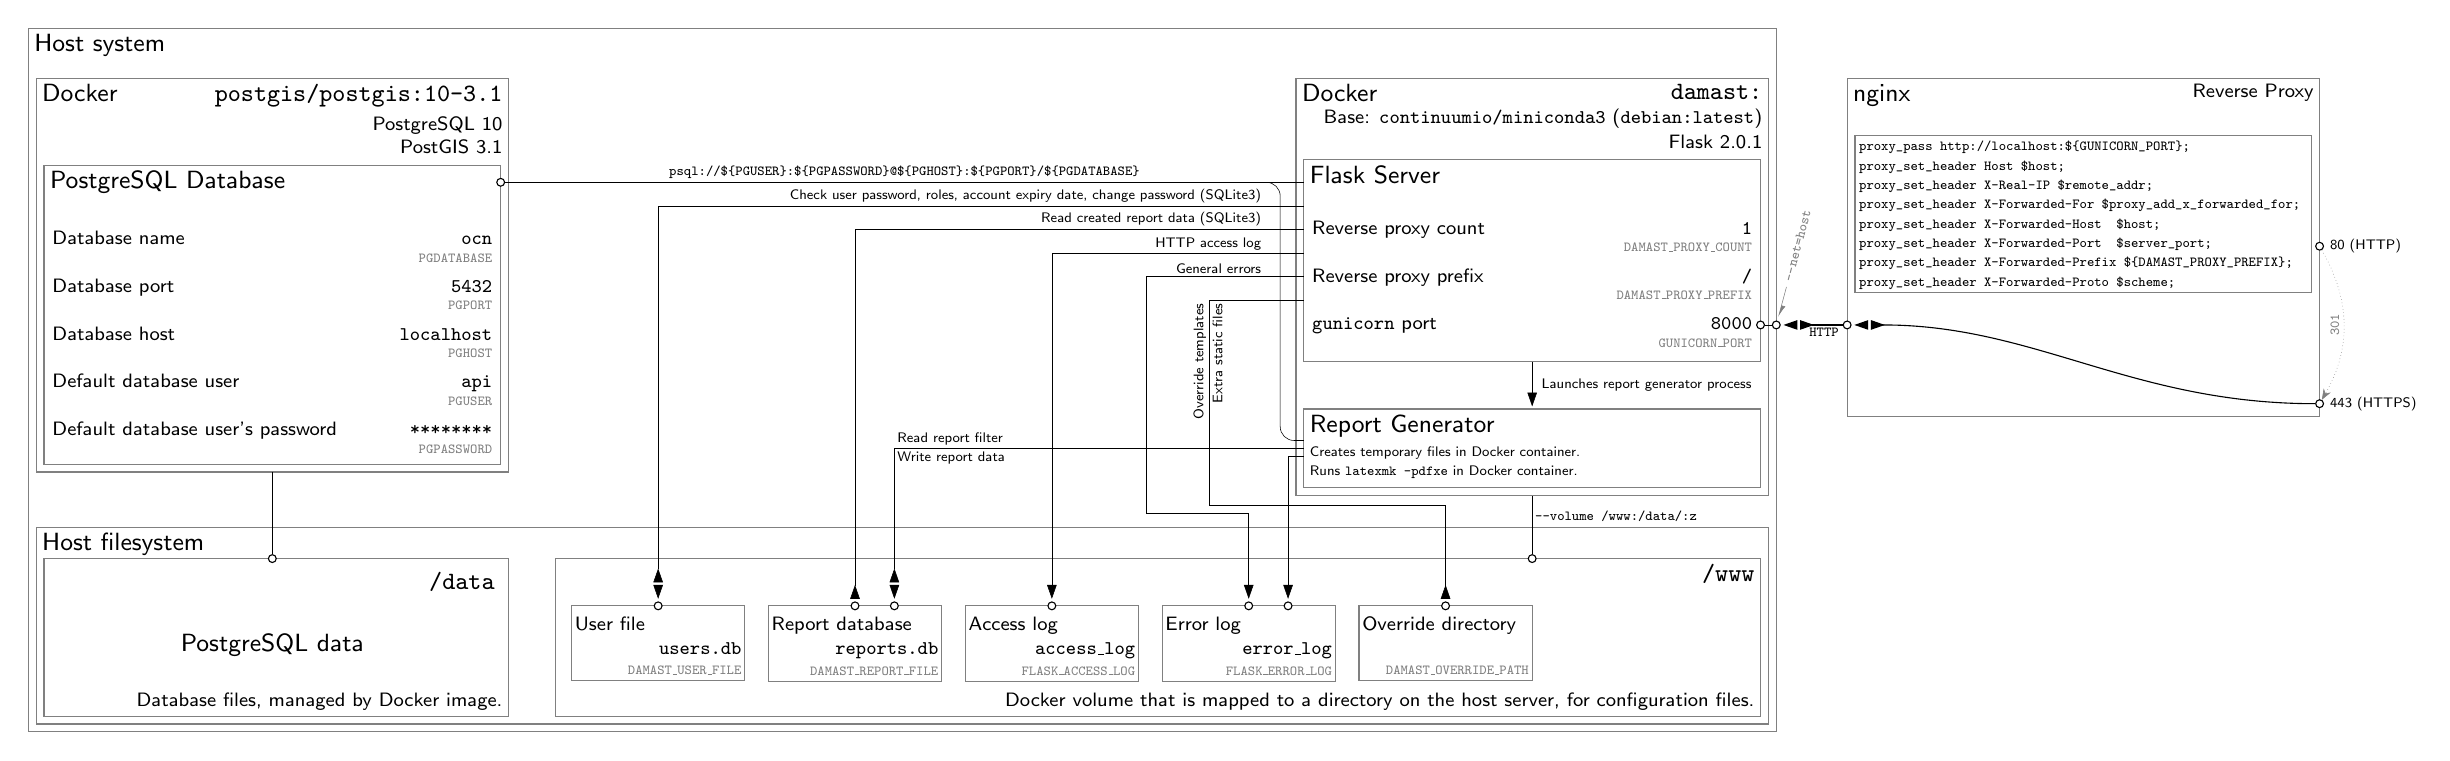
\begin{tikzpicture}
  \draw [frame] (0,0) coordinate (psql-docker-north-west)
    rectangle (6,-5) coordinate (psql-docker-south-east);
  \node [anchor=north west,inner sep=2pt] at (0,0) { \small Docker };
  \node [anchor=north east,inner sep=2pt] (docker-imagename) at (6,0) {\small \texttt{postgis/postgis:10-3.1}};
  \node [anchor=north east,inner xsep=2pt,inner ysep=1pt] (docker-imagename-1) at (docker-imagename.south east) {\scriptsize PostgreSQL 10};
  \node [anchor=north east,inner xsep=2pt,inner ysep=1pt] (docker-imagename-2) at (docker-imagename-1.south east) {\scriptsize PostGIS 3.1};

  \draw [frame] ($ (docker-imagename-2.south east) + (-0.1, -0.1) $)
                      coordinate (psql-db-rect-north-east)
                      rectangle (0.1, -4.9);
  \path let \p1 = (psql-db-rect-north-east),
            \p2 = (psql-docker-north-west),
            \p3 = (psql-docker-south-east)
            in coordinate (psql-db-rect-north-west) at (0.1, \y1)
               coordinate (psql-docker-south-west) at (\x2, \y3)
               coordinate (psql-docker-south) at ($ (psql-docker-south-west)!0.5!(psql-docker-south-east) $);
  \node [anchor = north west, inner sep=2pt] (psql-dblabel) at (psql-db-rect-north-west) {\small PostgreSQL Database};

  \coordinate (tmp) at ($ (psql-dblabel.south west) + (0.1,-0.2) $);
  \foreach \name/\label/\value/\varname in {
    dbname/{Database name}/ocn/PGDATABASE,
    dbport/{Database port}/5432/PGPORT,
    dbhost/{Database host}/localhost/PGHOST,
    dbuser/{Default database user}/api/PGUSER,
    dbpassword/{Default database user's password}/********/PGPASSWORD%
  } {
    \node [anchor=north west,inner sep=0] (psql-\name-label) at ($ (tmp) + (0,-0.2) $) { \scriptsize \label \phantom{Iq} };
    \path let \p1 = (psql-\name-label.north) in coordinate (tmp) at (5.8, \y1);
    \path let \p1 = (psql-\name-label.west) in coordinate (psql-\name-border) at (5.9, \y1);
    \node [anchor=north east,inner sep=0] (psql-\name) at (tmp) { \scriptsize \phantom{Iq}\texttt{\value} };
    \node [anchor=north east,inner sep=0,color=black!50] (psql-\name-var) at ($ (psql-\name.south east) + (0,-0.05) $) { \tiny \texttt{\varname} };
    \path let \p1 = (psql-\name-var.south) in coordinate (tmp) at (0.2, \y1);
  }


  \begin{scope}[xshift=16cm]
    \draw [frame] (0,0) coordinate (damast-docker-north-west)
                            rectangle (6,-5.3)
                            coordinate (damast-docker-south-east);
    \node [anchor=north west,inner sep=2pt] at (0,0) { \small Docker };
    \node [anchor=north east,inner sep=2pt] (docker-imagename) at (6,0) {\small \texttt{damast:\damastversion}};
    \node [anchor=north east,inner xsep=2pt,inner ysep=1pt] (docker-imagename-1) at (docker-imagename.south east) {\scriptsize Base: \texttt{continuumio/miniconda3} (\texttt{debian:latest}) };
    \node [anchor=north east,inner xsep=2pt,inner ysep=1pt] (docker-imagename-2) at (docker-imagename-1.south east) {\scriptsize Flask 2.0.1 };

    \draw [frame] ($ (docker-imagename-2.south east) + (-0.1, -0.1) $)
                        coordinate (damast-rect-north-east)
                        rectangle (0.1, -3.6)
                        coordinate (damast-rect-south-west);
    \path let \p1 = (damast-rect-north-east),
              \p2 = (damast-rect-south-west)
          in coordinate (damast-rect-north-west) at (\x2, \y1)
             coordinate (damast-rect-south-east) at (\x1, \y2)
             coordinate (reporter-rect-south-east) at (\x1, -5.2);
    \node [anchor = north west, inner sep=2pt] (damast-label) at (damast-rect-north-west) {\small Flask Server };

    \coordinate (tmp) at ($ (damast-label.south west) + (0.1,-0.2) $);
    \foreach \name/\label/\value/\varname in {
      proxycount/{Reverse proxy count}/1/DAMAST\_PROXY\_COUNT,
      proxyprefix/{Reverse proxy prefix}/{/}/DAMAST\_PROXY\_PREFIX,
      gunicorn/{\texttt{gunicorn} port}/8000/GUNICORN\_PORT,
    } {
      \node [anchor=north west,inner sep=0] (psql-\name-label) at ($ (tmp) + (0,-0.2) $) { \scriptsize \label \phantom{Iq} };
      \path let \p1 = (psql-\name-label.north) in coordinate (tmp) at (5.8, \y1);
      \node [anchor=north east,inner sep=0] (psql-\name) at (tmp) { \scriptsize \phantom{Iq}\texttt{\value} };
      \node [anchor=north east,inner sep=0,color=black!50] (psql-\name-var) at ($ (psql-\name.south east) + (0,-0.05) $) { \tiny \texttt{\varname} };
      \path let \p1 = (psql-\name-var.south) in coordinate (tmp) at (0.2, \y1);
    }


    \draw [frame] ($ (damast-rect-south-west) + (0, -0.6) $)
                        coordinate (reporter-rect-north-west)
                        rectangle (reporter-rect-south-east);

    \path let \p1 = (reporter-rect-north-west),
              \p2 = (reporter-rect-south-east)
          in coordinate (reporter-rect-north-east) at (\x2, \y1)
             coordinate (reporter-rect-south-west) at (\x1, \y2);
    \coordinate (reporter-north) at ($ (reporter-rect-north-west)!0.5!(reporter-rect-north-east) $);
    \coordinate (reporter-west) at ($ (reporter-rect-north-west)!0.5!(reporter-rect-south-west) $);
    \coordinate (damast-flask-south) at ($ (damast-rect-south-west)!0.5!(damast-rect-south-east) $);

    \node [anchor = north west, inner sep=2pt] (reporter-label) at (reporter-rect-north-west) {\small Report Generator };
    \node [anchor=north west,inner xsep=2pt,inner ysep=1pt] (tmpx) at (reporter-label.south west) {\tiny Creates temporary files in Docker container. };
    \node [anchor=north west,inner xsep=2pt,inner ysep=1pt] at (tmpx.south west) {\tiny Runs \verb!latexmk -pdfxe! in Docker container. };
  \end{scope}

  \begin{scope}[yshift=-6.2cm]
    \draw [frame] (0,0.5) coordinate (hostfs-north-west)
    rectangle (22,-2)
    coordinate (hostfs-south-east);
    \node [anchor=north west,inner sep=2pt] at (0,0.5) { \small Host filesystem };

    \begin{scope}[xshift=0cm]
      \draw [frame] (0.1,0.1) rectangle (6,-1.9) coordinate (hostfs1-south-east);
      \node [anchor=north east,inner sep=2pt] (host-fs-path) at (5.9,0) {\small \texttt{/data}};
      \coordinate (hostfs1-north) at (3,0.1);

      \node (hostfs1-label) at (3,-1) { \small PostgreSQL data };
      \node [anchor=south east,inner sep=2pt] at (hostfs1-south-east) { \scriptsize Database files, managed by Docker image. };

      \node [circle,fill=white,draw=black,inner sep=1pt] (hostfs1-node) at (hostfs1-north) {};
    \end{scope}

    \begin{scope}[xshift=6.5cm]
      \draw [frame] (0.1,0.1) coordinate (hostfs2-north-west)
      rectangle (15.4,-1.9)
      coordinate (hostfs2-south-east);
      \node [anchor=north east,inner sep=2pt] (host-fs-path) at (15.4,0.1) {\small \texttt{/www}};
      \path let \p1 = (hostfs2-south-east) in coordinate (hostfs2-south-west) at (0.1, \y1);
      \node [anchor=south east,inner sep=2pt] at (hostfs2-south-east) { \scriptsize Docker volume that is mapped to a directory on the host server, for configuration files. };

      \coordinate (tmp) at (0,-0.5);
      \foreach \name/\title/\label/\varname in {
        userdb/User file/users.db/DAMAST\_USER\_FILE,
        report/Report database/reports.db/DAMAST\_REPORT\_FILE,
        access/Access log/access\_log/FLASK\_ACCESS\_LOG,
        error/Error log/error\_log/FLASK\_ERROR\_LOG,
        override/Override directory//DAMAST\_OVERRIDE\_PATH%
      } {
        \coordinate (nw) at ($ (tmp) + (0.3,0) $);
        \coordinate (ne) at ($ (nw) + (2.2,0) $);

        \node [inner sep=1pt,anchor=north west,yshift=-3pt] (\name-title) at (nw) { \scriptsize \title\phantom{Iq} };
        \path let \p1 = (ne), \p2 = (\name-title.south east) in coordinate (tmp) at (\x1, \y2);

        \node [inner sep=1pt,anchor=north east] (\name-label) at (tmp) { \scriptsize \phantom{Iq}\texttt{\label} };
        \node [inner sep=1pt,anchor=north east,color=black!50] (\name-var) at (\name-label.south east) { \tiny \phantom{Iq}\texttt{\varname} };

        \path let \p1 = (ne), \p2 = (\name-var.south east) in coordinate (se) at (\x1, \y2);

        \draw [frame] (nw) rectangle (se);
        \node [circle,fill=white,draw=black,inner sep=1pt] (hostfs-\name-node) at ($ (nw)!0.5!(ne) $) {};

        \coordinate (tmp) at (ne);
      }
    \end{scope}
  \end{scope}

  \path let \p1 = (psql-gunicorn),
            \p2 = (damast-rect-south-east)
        in coordinate (damast-port) at (\x2, \y1);

  \begin{scope}[xshift=23cm]
    \draw [frame] (0,0) coordinate (nginx-north-west)
                            rectangle (6,-4.3)
                            coordinate (nginx-south-east);

    \path let \p1 = (damast-port),
              \p2 = (nginx-north-west),
              \p3 = (nginx-south-east)
          in coordinate (nginx-inner-port) at (\x2, \y1)
             coordinate (nginx-south-west) at (\x2, \y3)
             coordinate (nginx-north-east) at (\x3, \y2)
             coordinate (nginx-outer-port) at (\x3, \y1)
             coordinate (nginx-outer-80) at ($ (nginx-outer-port) + (0,1) $)
             coordinate (nginx-outer-443) at ($ (nginx-outer-port) + (0,-1) $);

    \node [anchor=north west,inner sep=2pt] (tmp) at (nginx-north-west) { \small nginx };
    \node [anchor=north east,inner sep=2pt] at (nginx-north-east) { \scriptsize Reverse Proxy };

    \node [circle,fill=white,draw=black,inner sep=1pt] (nginx-inner) at (nginx-inner-port) {};
    \node [circle,fill=white,draw=black,inner sep=1pt] (nginx-80) at (nginx-outer-80) {};
    \node [circle,fill=white,draw=black,inner sep=1pt] (nginx-443) at (nginx-outer-443) {};

    \node [inner sep=2pt,anchor=west] at (nginx-80.east) { \tiny 80 (HTTP) };
    \node [inner sep=2pt,anchor=west] at (nginx-443.east) { \tiny 443 (HTTPS) };

    \draw [bend left,very thin,gray,densely dotted,-Stealth] (nginx-80) edge (nginx-443);
    \node [gray,anchor=north,inner sep=1pt,rotate=90,yshift=-0.1cm] at ($ (nginx-80)!0.5!(nginx-443) $) {\tiny \texttt{301}};

    \draw [read write] (nginx-443.west) to[out=-180,in=0] (nginx-inner.east);

    \coordinate (nginx-conf-nw) at ($ (tmp.south west) + (0.1,-0.3) $);
    \path let \p1 = (nginx-conf-nw),
              \p2 = (nginx-south-east)
          in coordinate (nginx-conf-nex) at (\x2, \y1)
          coordinate (nginx-conf-ne) at ($ (nginx-conf-nex) + (-0.1, 0) $);
    \node [inner sep=0] (tmp) at (nginx-conf-nw) {};

    \node [inner xsep=2pt,inner ysep=1pt,anchor=north west] (tmp) at (tmp.south west) { \tiny\verb!proxy_pass http://localhost:${GUNICORN_PORT};! };
    \node [inner xsep=2pt,inner ysep=1pt,anchor=north west] (tmp) at (tmp.south west) { \tiny\verb!proxy_set_header Host $host;! };
    \node [inner xsep=2pt,inner ysep=1pt,anchor=north west] (tmp) at (tmp.south west) { \tiny\verb!proxy_set_header X-Real-IP $remote_addr;! };
    \node [inner xsep=2pt,inner ysep=1pt,anchor=north west] (tmp) at (tmp.south west) { \tiny\verb!proxy_set_header X-Forwarded-For $proxy_add_x_forwarded_for;! };
    \node [inner xsep=2pt,inner ysep=1pt,anchor=north west] (tmp) at (tmp.south west) { \tiny\verb!proxy_set_header X-Forwarded-Host  $host;! };
    \node [inner xsep=2pt,inner ysep=1pt,anchor=north west] (tmp) at (tmp.south west) { \tiny\verb!proxy_set_header X-Forwarded-Port  $server_port;! };
    \node [inner xsep=2pt,inner ysep=1pt,anchor=north west] (tmp) at (tmp.south west) { \tiny\verb!proxy_set_header X-Forwarded-Prefix ${DAMAST_PROXY_PREFIX};! };
    \node [inner xsep=2pt,inner ysep=1pt,anchor=north west] (tmp) at (tmp.south west) { \tiny\verb!proxy_set_header X-Forwarded-Proto $scheme;! };

    \path let \p1 = (nginx-conf-ne),
              \p2 = (tmp.south)
          in coordinate (nginx-conf-se) at (\x1, \y2);
    \draw [frame] (nginx-conf-nw) rectangle (nginx-conf-se);
  \end{scope}

  \path let \p1 = (psql-db-rect-north-east),
            \p2 = (psql-dblabel.east)
        in coordinate (psql-borderpos) at (\x1, \y2);
  \node [circle,fill=white,draw=black,inner sep=1pt] (psql-dbport-bordericon) at (psql-borderpos) {};
  \path let \p1 = (psql-dbport-bordericon),
            \p2 = (damast-rect-north-west)
        in coordinate (damast-borderpos) at (\x2, \y1);

  \foreach \delta in {1,...,5} {
    \coordinate (damast-borderpos-\delta) at ($ (damast-borderpos) + (0,\delta * -0.3) $);
    \coordinate (damast-borderpos-\delta-label) at ($ (damast-borderpos-\delta) + (-0.5,0) $);
  }

  \draw [very thin,read write] (damast-borderpos-1) -| (hostfs-userdb-node.north);
  \node [anchor=south east,inner sep=1pt] at (damast-borderpos-1-label) { \tiny Check user password, roles, account expiry date, change password (SQLite3) };
  \draw [very thin,read] (damast-borderpos-2) -| (hostfs-report-node.north);
  \node [anchor=south east,inner sep=1pt] at (damast-borderpos-2-label) { \tiny Read created report data (SQLite3) };
  \draw [very thin,write] (damast-borderpos-3) -| (hostfs-access-node.north);
  \node [anchor=south east,inner sep=1pt] at (damast-borderpos-3-label) { \tiny HTTP access log };
  \draw [very thin,write] (damast-borderpos-4) -- ++(-2,0) -- ++(0,-3) -| (hostfs-error-node.north);
  \node [anchor=south east,inner sep=1pt] at (damast-borderpos-4-label) { \tiny General errors };

  \coordinate (damast-borderpos-5-label) at ($ (damast-borderpos-5) + (-1.2,0) $);
  \draw [very thin,read] (damast-borderpos-5) -- (damast-borderpos-5-label) -- ++(0,-2.6) -| (hostfs-override-node);
  \node [anchor=south east,inner sep=1pt,rotate=90] at (damast-borderpos-5-label) {\tiny Override templates};
  \node [anchor=north east,inner sep=1pt,rotate=90] at (damast-borderpos-5-label) {\tiny Extra static files};

  \draw (damast-borderpos) -- (psql-dbport-bordericon.east)
      node [midway,above,inner ysep=1pt] {\tiny \verb!psql://${PGUSER}:${PGPASSWORD}@${PGHOST}:${PGPORT}/${PGDATABASE}!};

  \draw (psql-docker-south) -- (hostfs1-node.north);

  \node [anchor=south west,inner sep=2pt,xshift=-0.1cm,yshift=0.2cm] (host-label) at (psql-docker-north-west) { \small Host system };
  \draw [frame] (host-label.north west) rectangle ($ (hostfs-south-east) + (0.1,-0.1) $)
    coordinate (hostsystem-south-east);

  \path let \p1 = (damast-docker-south-east),
            \p2 = (damast-docker-north-west)
        in coordinate (damast-docker-south-west) at (\x2, \y1)
           coordinate (damast-docker-south) at ($ (damast-docker-south-east)!0.5!(damast-docker-south-west) $);

  \path let \p1 = (damast-docker-south),
            \p2 = (hostfs2-north-west)
        in coordinate (www-hostfs-top) at (\x1, \y2);

  \node [circle,fill=white,draw=black,inner sep=1pt] (hostfs2-node) at (www-hostfs-top) {};
  \draw [very thin] (hostfs2-node.north) -- (damast-docker-south)
    node [inner sep=1pt,anchor=west,pos=0.65] { \tiny \texttt{--volume /www:/data/:z} };

  \draw [very thin,write] (damast-flask-south) -- (reporter-north) node [midway,anchor=west] { \tiny Launches report generator process };
  \coordinate (rep-west-1) at ($ (reporter-west) + (0,0.1) $);
  \coordinate (rep-west-2) at ($ (reporter-west) + (0,-0.1) $);
  \draw [very thin,rounded corners=5pt] (rep-west-1) -- ++(-0.3,0) |- (psql-dbport-bordericon.east);

  \node [circle,fill=white,draw=black,inner sep=1pt] (report-writenode) at ($ (hostfs-report-node) + (0.5,0) $) {};
  \draw [very thin,read write] (reporter-west) -| (report-writenode)
    node [midway,inner sep=1pt,anchor=south west] { \tiny Read report filter }
    node [midway,inner sep=1pt,anchor=north west] { \tiny Write report data };

  \node [circle,fill=white,draw=black,inner sep=1pt] (report-writenode2) at ($ (hostfs-error-node) + (0.5,0) $) {};
  \draw [very thin,write] (rep-west-2) -| (report-writenode2);

  \path let \p1 = (hostsystem-south-east),
            \p2 = (damast-port)
        in coordinate (damast-port-outer) at (\x1, \y2);

  \node [circle,fill=white,draw=black,inner sep=1pt] (damast-httpport) at (damast-port) {};
  \node [circle,fill=white,draw=black,inner sep=1pt] (damast-httpport-outer) at (damast-port-outer) {};
  \draw [very thin] (damast-httpport.east) -- (damast-httpport-outer.west);
  \draw [read write] (nginx-inner.west) -- (damast-httpport-outer)
    node [pos=0.3,below,inner sep=1pt] { \tiny \verb!HTTP! };

  \coordinate (tmp) at ($ (damast-port)!0.5!(damast-port-outer) $);

  \node [anchor=west,rotate=75,inner xsep=2pt,color=gray] (tmp) at ($ (damast-port-outer) + (75:0.5) $) { \tiny \verb!--net=host! };
  \draw [very thin,gray,-{Latex[left]},shorten >= 3pt] (tmp) -- (damast-port-outer);
\end{tikzpicture}
\end{document}
